\subsection{Lines}
\noindent
A straight line is probably the simplest 3D VVF. We can form any straight line using a point that the line passes through and the direction veto of the line.\\
Letting $P$ be the point and $\vec{v}$ be the direction, a straight line has the form $\vec{r}(t)=\vec{P}+t\vec{v}$, where $\vec{P}$ is the vector with components the same as $P$. The function's output starts at $\vec{P}$ when $t=0$ and moves in the direction of $\vec{v}$ as $t$ increases.

% It'd be nice if we could get this image to fit on the above page
\begin{figure}[h]
	\centering
	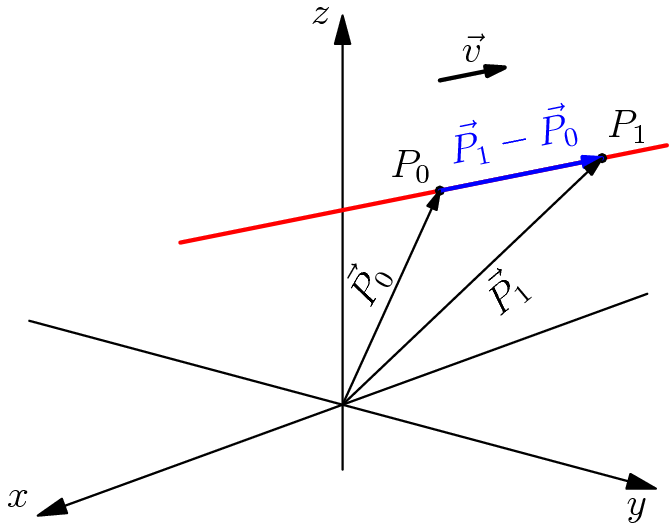
\includegraphics[scale=0.33]{Images/vectorValuedFunctions/VectorLine}
\end{figure}

\noindent
A line can also be formed using two points. To find the equation of the line in this case, let $\vec{v}$ be the vector connecting the two points, and let $\vec{P}$ be a vector point from the origin to one of the two points. We now have an origin point and direction and can write our function as $\vec{r}(t)=\vec{P_0}+t\left(\vec{P_1}-\vec{P_0}\right)$. Where $P_0$ and $P_1$ are the two points on the line.